\section{Change of assumptions}

There have been no significant changes from the assumptions delineated in our initial report. Consequently, we are adhering to our original plan.

\section{Architecture of your module}
The module \texttt{gossip} has been developed using the Golang programming language. It relies heavily on Go features like goroutines, Go channels, and multiple Go libraries. 

\subsection{The whole picture}

As the specification requires, the \texttt{gossip} module runs as two independent protocols: one API protocol and one P2P protocol. However, these two protocols share some data to fulfill the functionality of the module. 

\begin{figure}[H]
    \centering
    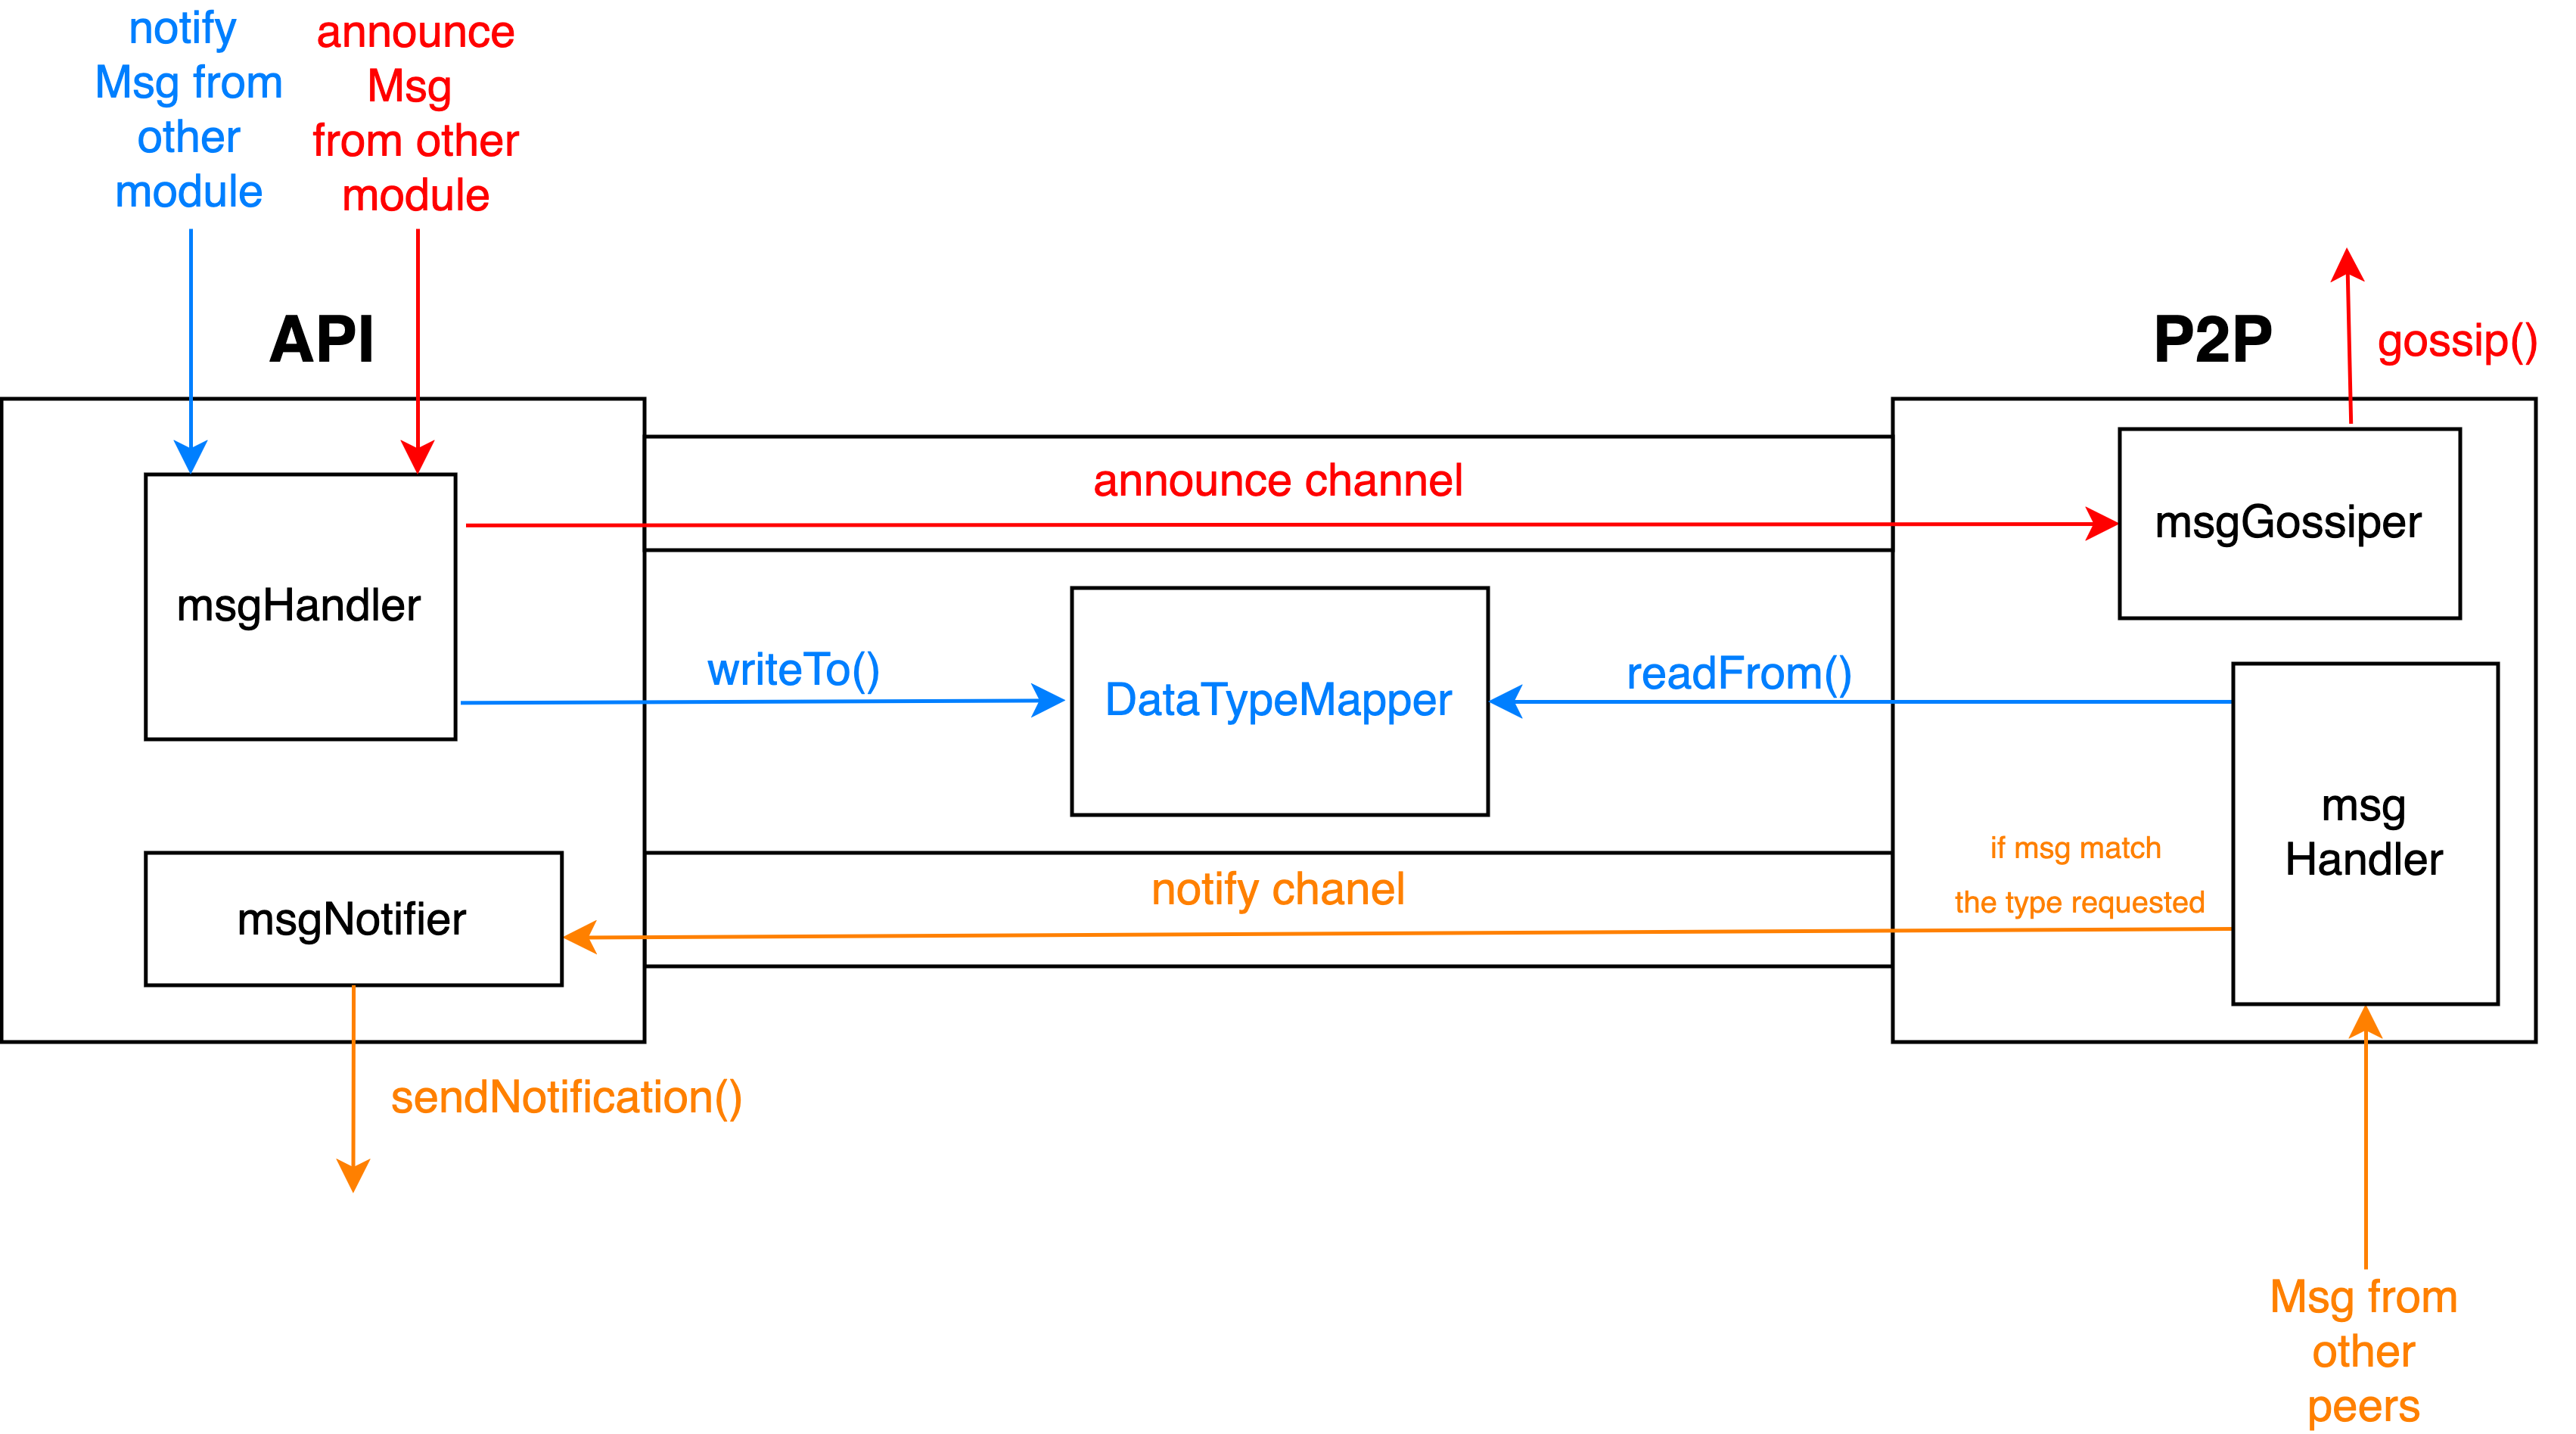
\includegraphics[width=0.7\textwidth]{pics/structure.png}
    \caption{Structure of the gossip module}
\end{figure}

\subsubsection{1. Announce messages Go channel}

To make the announce functionality work, we need an \textbf{announce Go channel}\footnote{Marked in red in Figure 1} shared between the two protocols. Whenever the API protocol receives an announce message from another module, it processes the message immediately and sends it to the P2P protocol through this channel. The P2P protocol has an announce message handler running on a goroutine that always listens to this channel. When it receives an announce request, it will gossip this message away. 

\begin{lstlisting}
announceMsgChan := make(chan enum.AnnounceMsg)
\end{lstlisting}

\subsubsection{2. Datatype mapper}

To make the notify functionality work, we need a \textbf{datatype mapper}\footnote{Marked in blue in Figure 1} shared between two protocols. Whenever API receives a notify message, it will write the message type that is valid into the mapper and hence should be propagated further. This datatype mapper will, of course, own a mutex that guarantees there is no race condition between the two protocols.

\begin{lstlisting}
type DatatypeMapper struct {
    mutex sync.RWMutex
    data  map[net.Addr]map[enum.Datatype]bool
}
\end{lstlisting}

\subsubsection{3. Notify messages Go channel}

Thanks to the datatype mapper, the P2P protocol can recognize which kind of message it should propagate. When it receives a new message, it will check if this message type was requested by any module by reading the datatype mapper. If that is the case, it sends this message through \textbf{notify message Go channel}\footnote{Marked in orange in Figure 1}. API protocol also has a running goroutine that constantly listens to this channel. It can get those messages from P2P and send corresponding notification messages to the module requesting them. 

\begin{lstlisting}
notifyMsgChan := make(chan enum.NotifyMsg)
\end{lstlisting}

\subsection{API}

The API operates by having the Server listen on a TCP address for connections, managed by Go's net package, and then forwarding these connections to a Handler. This Handler processes messages based on their type, using a custom logger for error reporting and Go's bytes and encoding/binary packages for message verification. It also routes messages to specific functions for handling different types, such as announcements, and communication across nodes.

Through seamless Server-Handler interaction, the API efficiently manages message processing and routing, maintaining system integrity across nodes. Go's concurrency tools, like goroutines and channels, enable handling of multiple connections, ensuring scalability and robustness for real-time, distributed communication.

\subsection{P2P}

\subsubsection{Bootstrapping strategy:}

Bootstrapping service is one of the important components of a P2P network that helps newly joined Node to get initial knowledge on current active peers in the network. 
In our current implementation, we use a static bootstrapping method to ensure that new nodes can join the network and connect to existing peers. The bootstrapping process involves the following steps:

\begin{enumerate}
    \item \textbf{Registration}: When a new node starts, it registers itself with the bootstrapper server. The server maintains a list of all registered peers.
    \item \textbf{Fetching Initial Peers}: After registration, the new node fetches an initial list of peers from the bootstrapper server. This list is used to establish initial connections and begin participating in the gossip protocol.
\end{enumerate}


\subsubsection{Gossip Node:}

The \texttt{GossipNode} implementation supports key functionalities for managing peer-to-peer communication. When a node starts, it registers with the bootstrapper server and fetches an initial list of peers to establish connections. When a node leaves, it announces its departure to its known peers, updating their peer lists.

The node disseminates information using a gossip protocol, spreading data such as new peers joining or leaving, and application messages to a random subset of peers. It processes and forwards incoming gossip messages to ensure widespread distribution. Nodes periodically exchange peer lists to maintain up-to-date network knowledge, dynamically adding new peers and removing inactive ones as necessary. 

A message handler is integrated into the \texttt{GossipNode}, which picks up the message type from the gossip message and handles it accordingly. This handler ensures that different types of messages (such as announcements, departures, data spreads, and peer list requests) are processed correctly and efficiently within the network.

\subsubsection{Properties}

The \texttt{GossipNode} has several properties. The fanout, set to n=2, determines the number of peers a node gossips to during each round. The gossip interval, set to m=5 seconds, specifies the frequency of gossip messages. The message cache prevents redundant processing by storing recently seen messages using a map data structure. The peers list, updated dynamically, maintains known peers for communication. The bootstrap URL is used for initial registration and fetching peers when nodes join the network.


\subsubsection{Gossip Message}

For efficient communication between peer, we define a structrue for Gossip Message:

\begin{itemize}
    \item \textbf{MESSAGE\_TYPE}:  Predefined type of gossip message.
    \item \textbf{TTL (Time to Live)}:  Get from API call, reduce by each hop.
    \item \textbf{RESERVED}: This field is reserved for future feature.
    \item \textbf{PAYLOAD}: Data gets from API calls.
\end{itemize}


\begin{figure}[H]
    \centering
    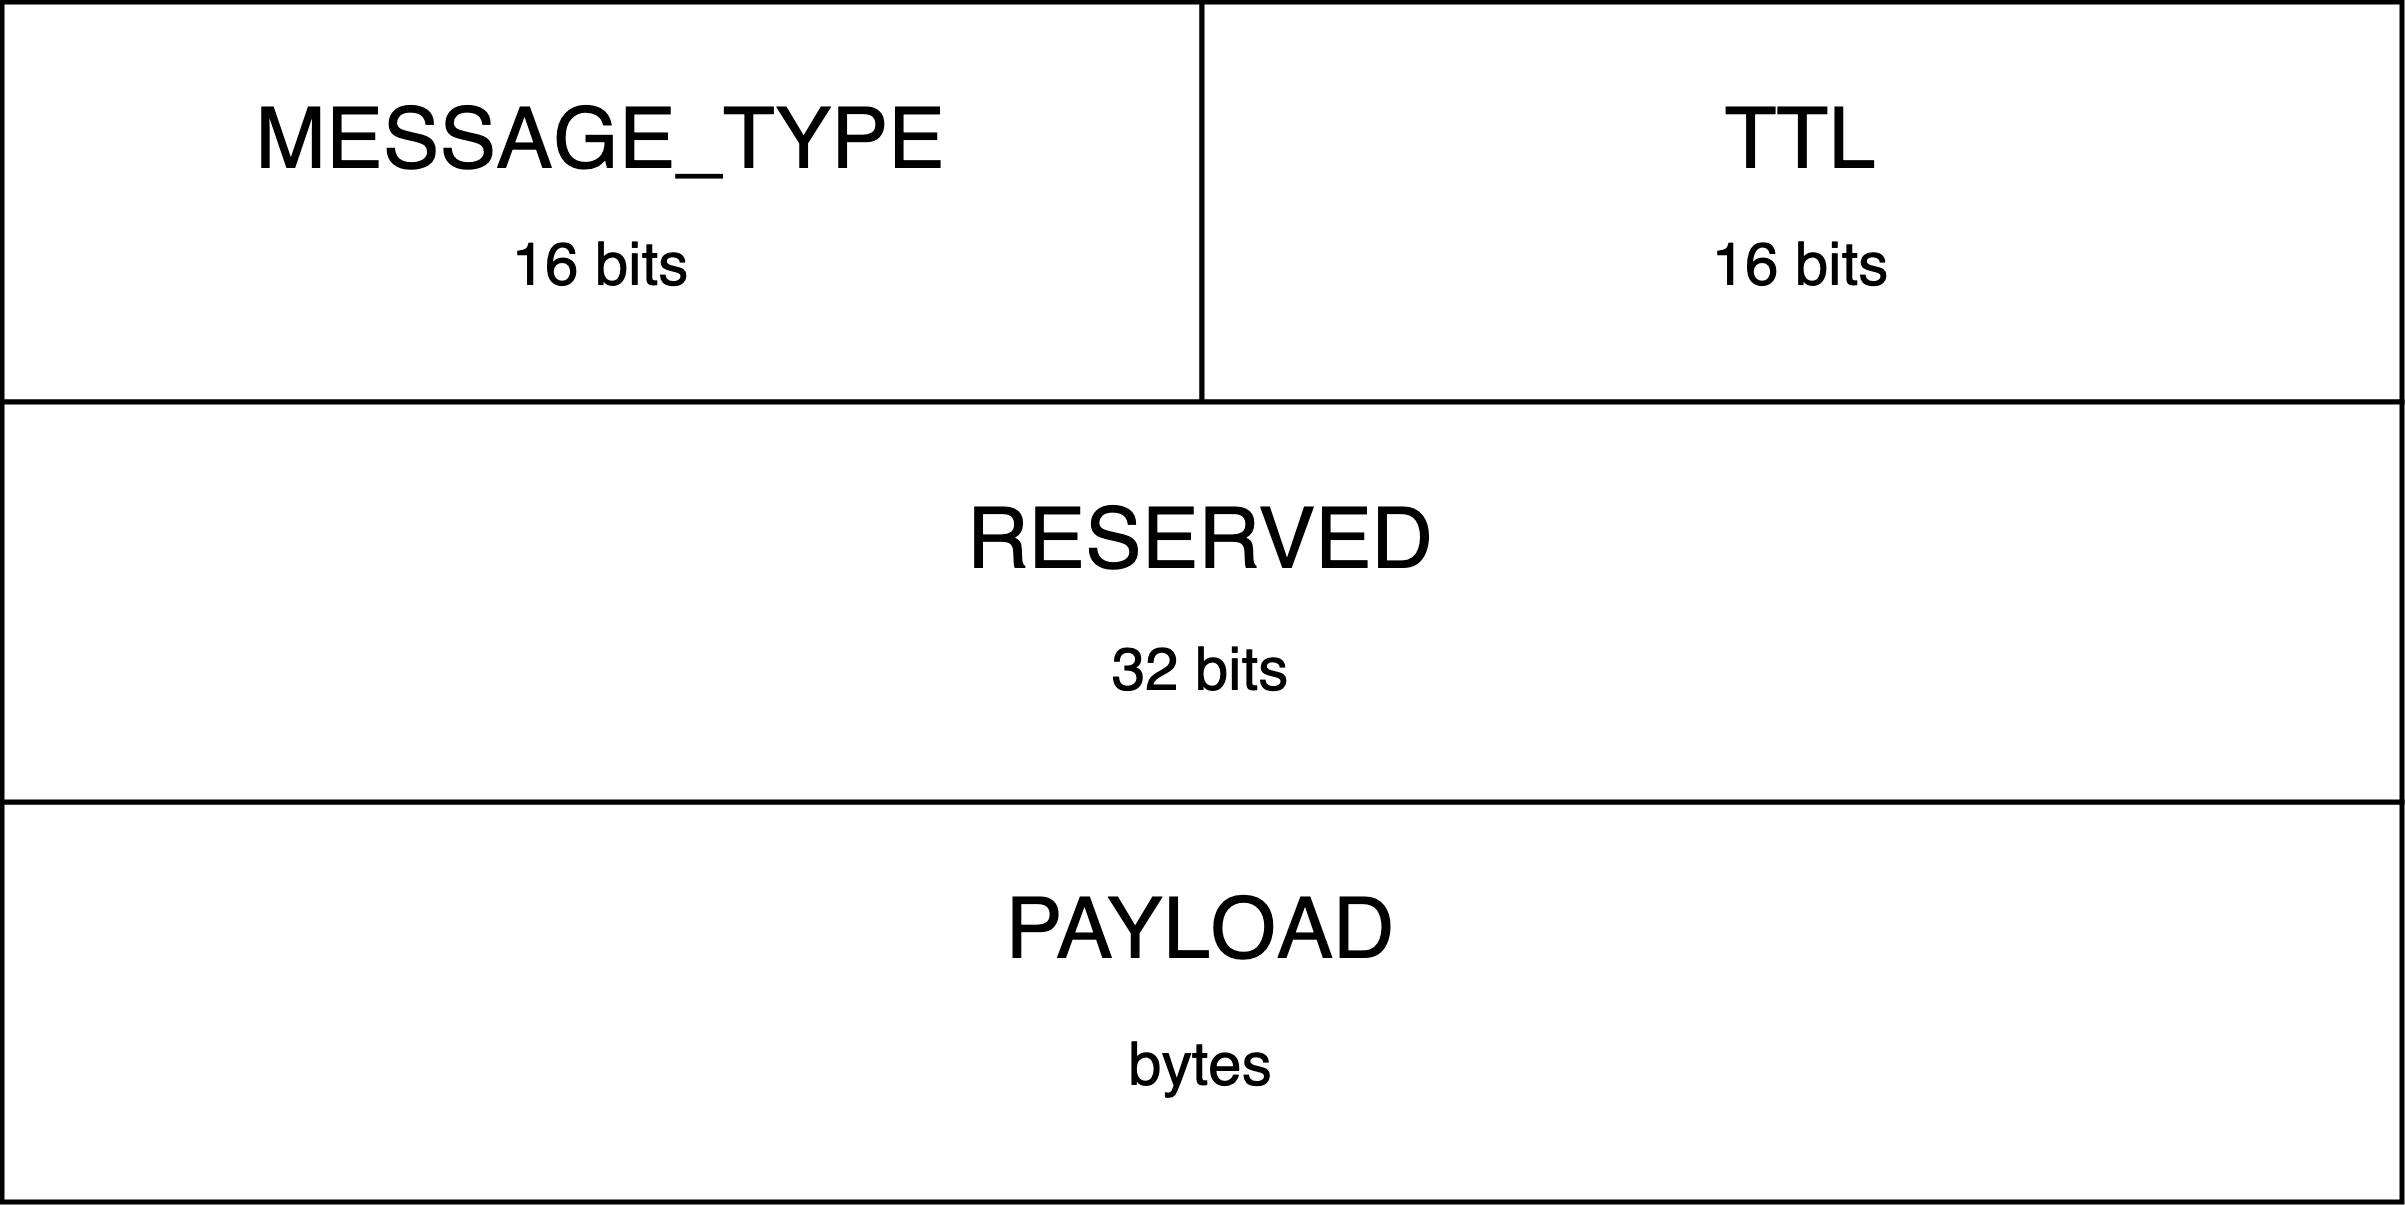
\includegraphics[width=0.45\textwidth]{pics/gossip.message.png}
    \caption{Gossip Message}
\end{figure}

\begin{itemize}
    \item \textbf{GossipMessageType}:
      
        \begin{itemize}
            \item \textbf{PEER\_ANNOUNCE}: Message announcing a new peer.
            \item \textbf{PEER\_LEAVE}: Message announcing a peer leaving the network.
            \item \textbf{DATA\_SPREAD}: Message containing data to be spread across the network.
            \item \textbf{PEER\_LIST\_REQUEST}: Message requesting the list of known peers.
            \item \textbf{PEER\_LIST\_RESPONSE}: Message containing the list of known peers.
        \end{itemize}
\end{itemize}

\section{Security Measures}

\subsection{Bootstrapper Proof-Of-Work (POW):}

For security of Bootstrapper, we implement POW mechanism for the registering process. To avoid sybil attack, we define target difficulty, which is the number of leading zeros of a hash that a peer should calculate in order to register successfully. Details of the process are belows:

\subsubsection{BOOTSTRAP INIT}

When a new peer opens a connection to Bootrapping Server, the server sends an \texttt{BOOTSTRAP \_INIT} message to the peer. This message contains a challenge and its target difficulty which this peer needs to use to calculate the hash.

\begin{figure}[H]
    \centering
    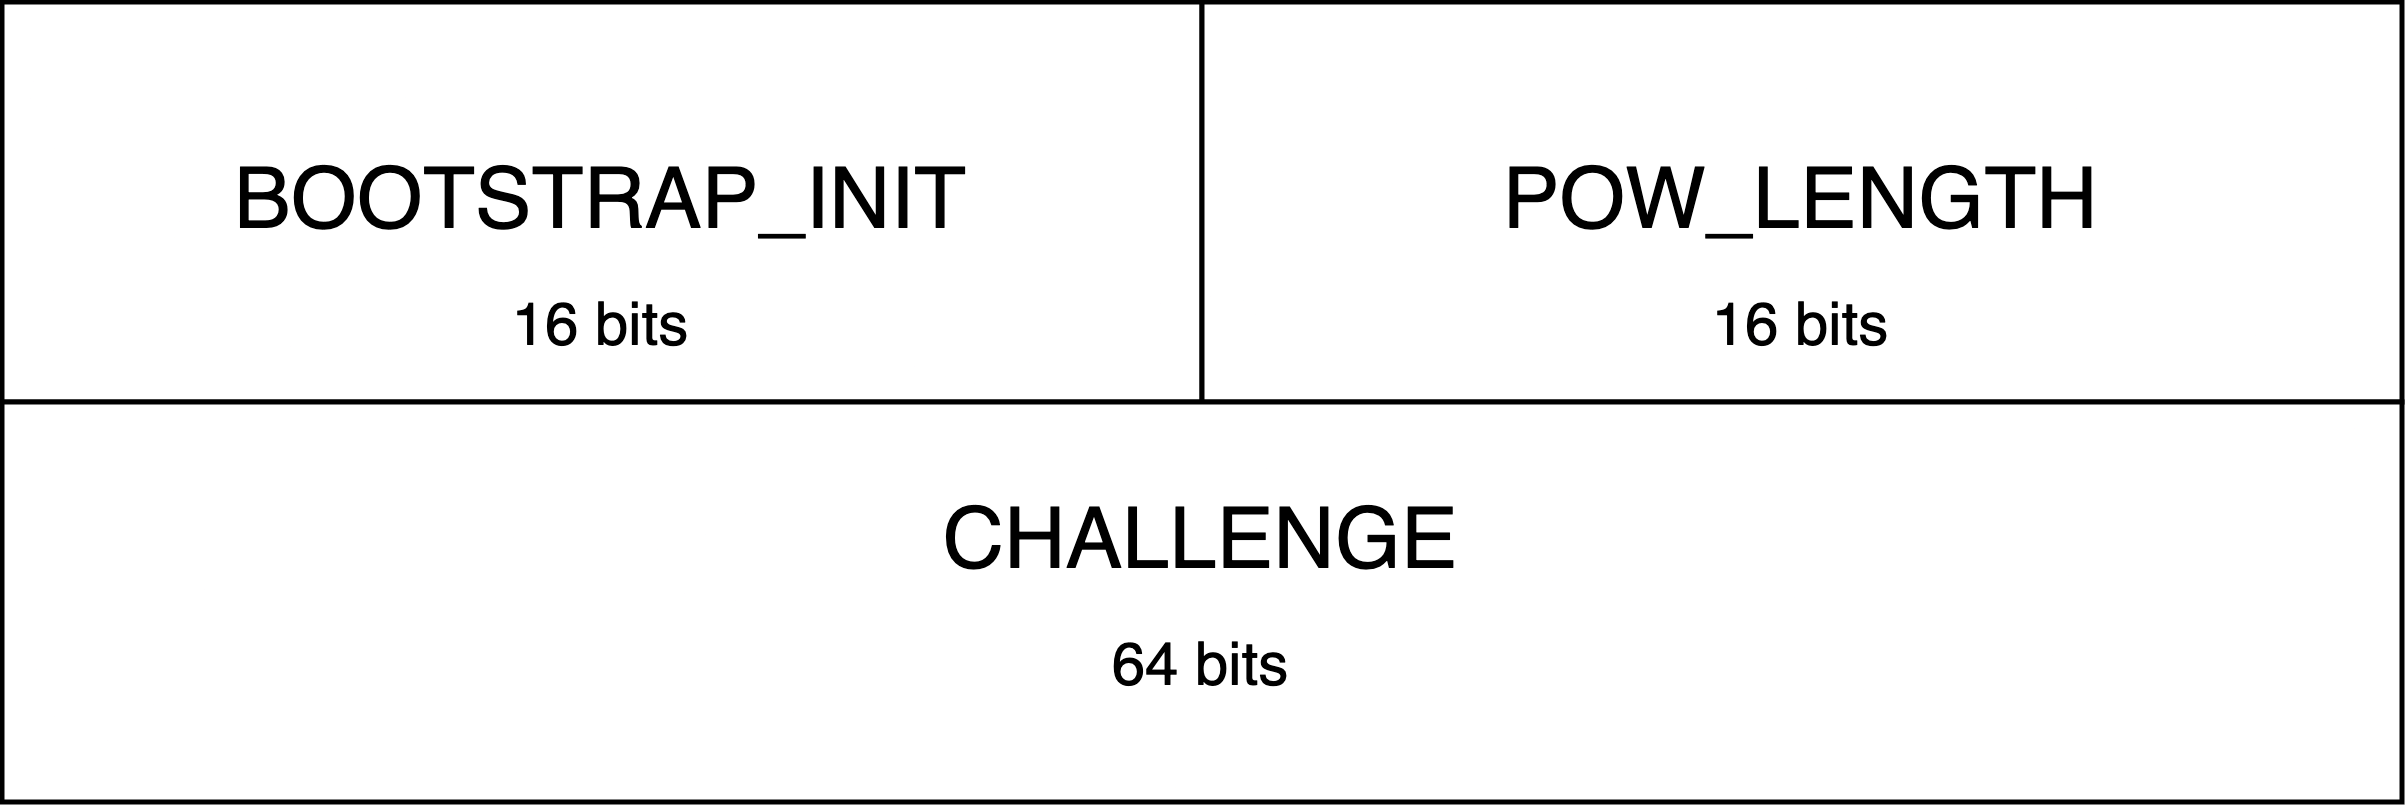
\includegraphics[width=0.45\textwidth]{pics/bootstrap.init.png}
    \caption{Bootstrap Init Message}
\end{figure}

\subsubsection{BOOTSTRAP REGISTER}

The peer calculates the SHA256 hash of the concatenation of the nonce (random number) and the challenge. If the resulting hash has the first n bits set to zeros (whereas n = target difficulty), then the peer can register by sending the \texttt{BOOTSTRAP\_REGISTER} message. If not, the nonce has to be changed to another random value and retried until one is found, which gives one of the required SHA256 values.

\begin{figure}[H]
    \centering
    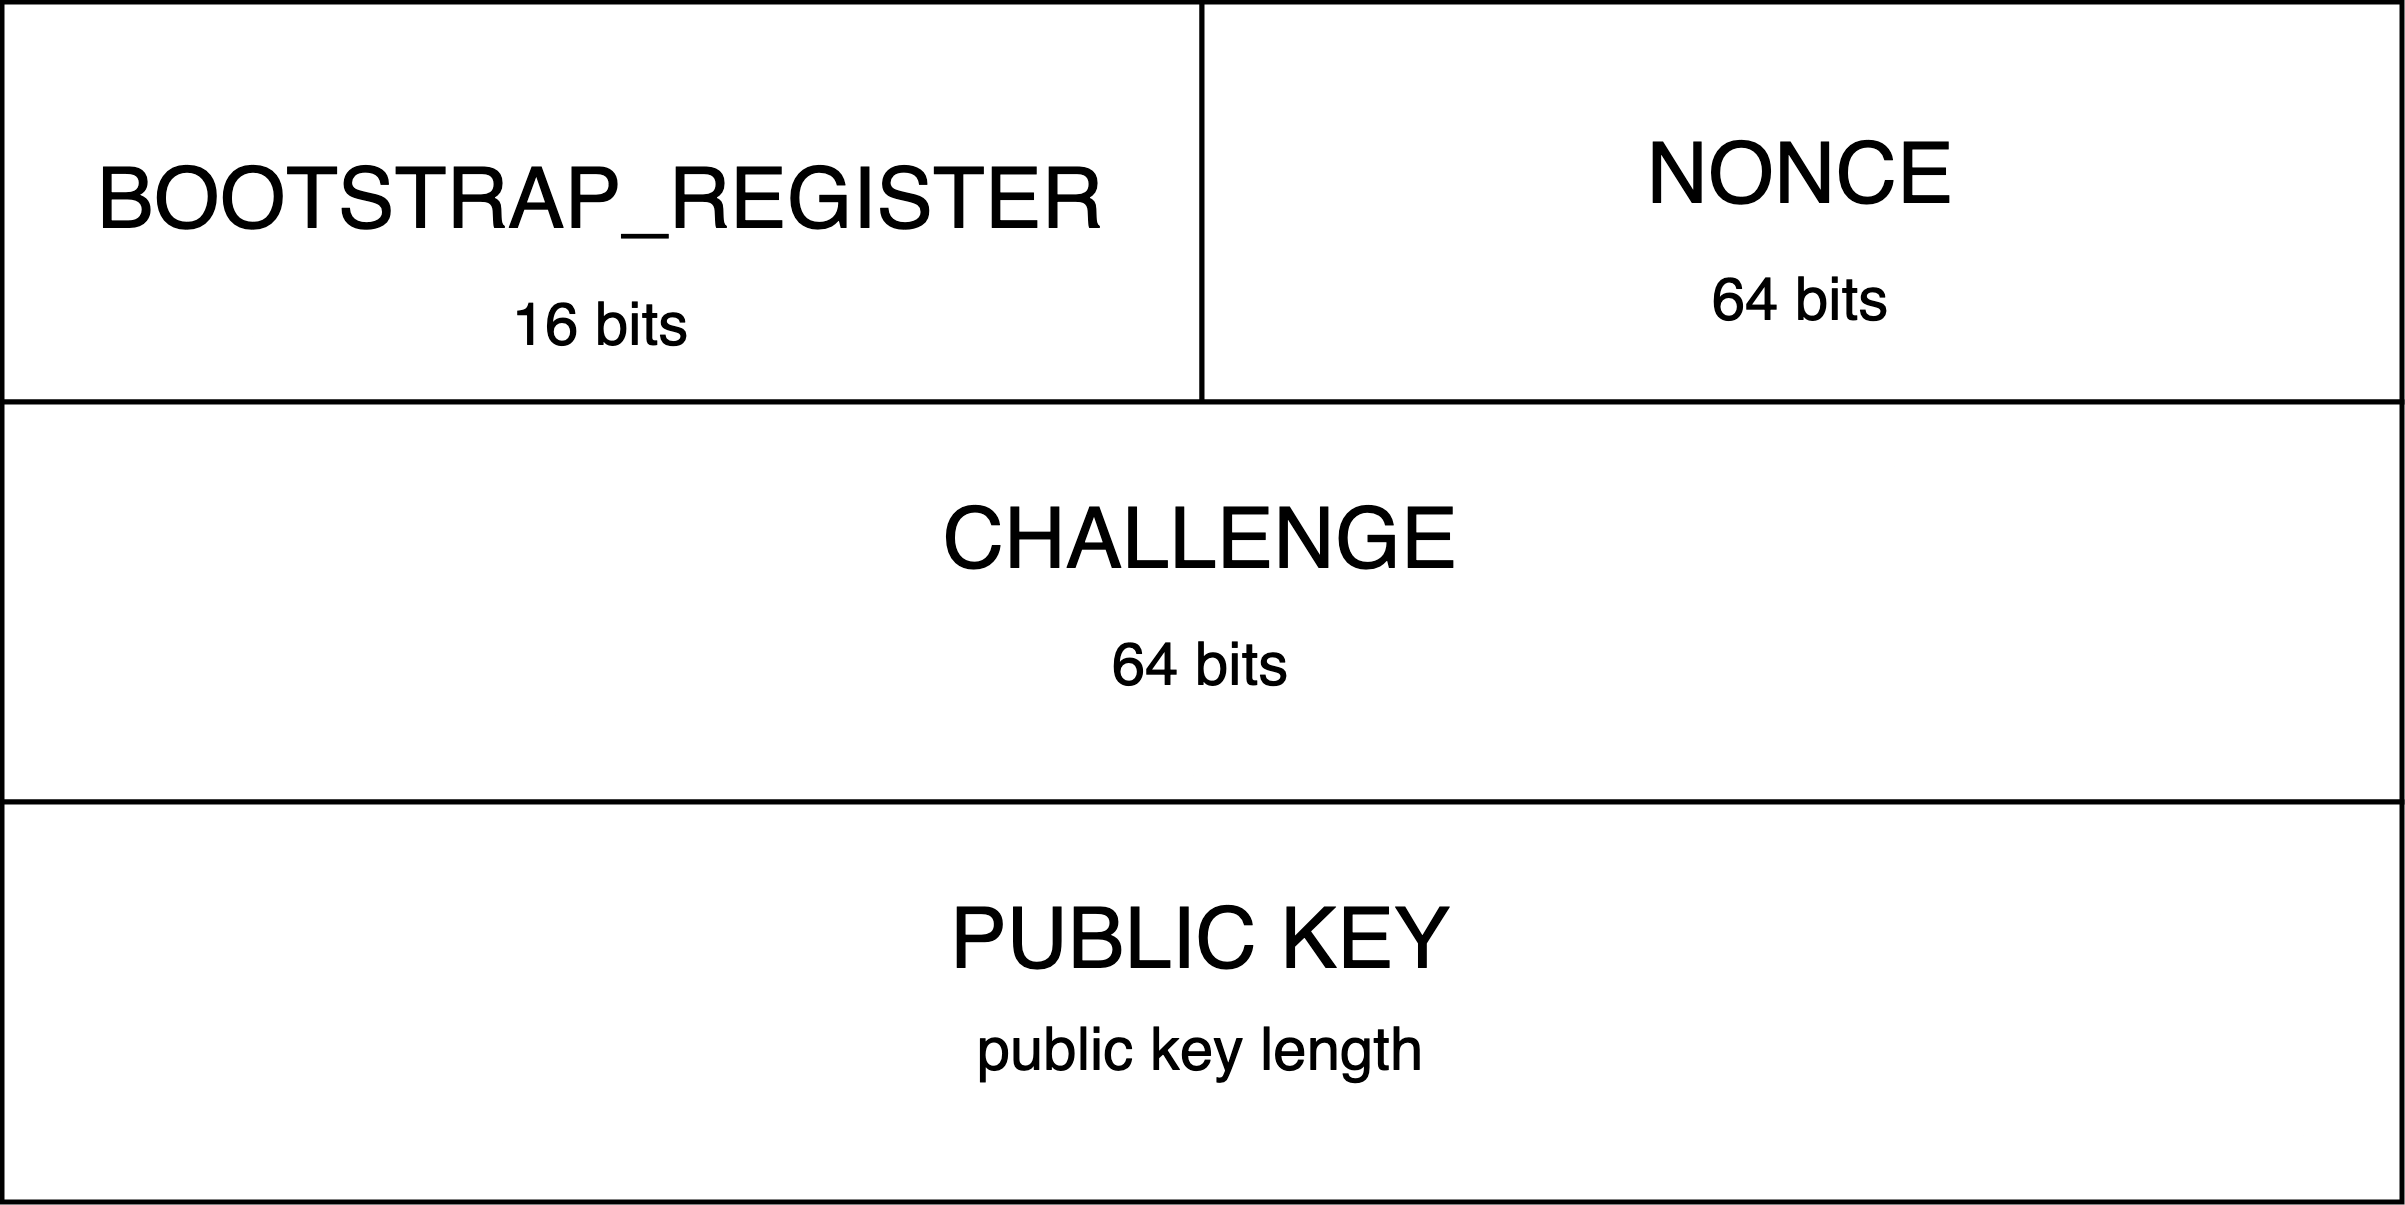
\includegraphics[width=0.45\textwidth]{pics/bootstrap.register.png}
    \caption{Bootstrap Register Message}
\end{figure}

\subsubsection{BOOTSTRAP SUCCESS}

If registeration is successful, meta data of the new peer got saved in local memory of the bootstrapping service and a \texttt{BOOTSTRAP\_SUCCESS} message is returned to the peer. The message also contains initial peer list.

\begin{figure}[H]
    \centering
    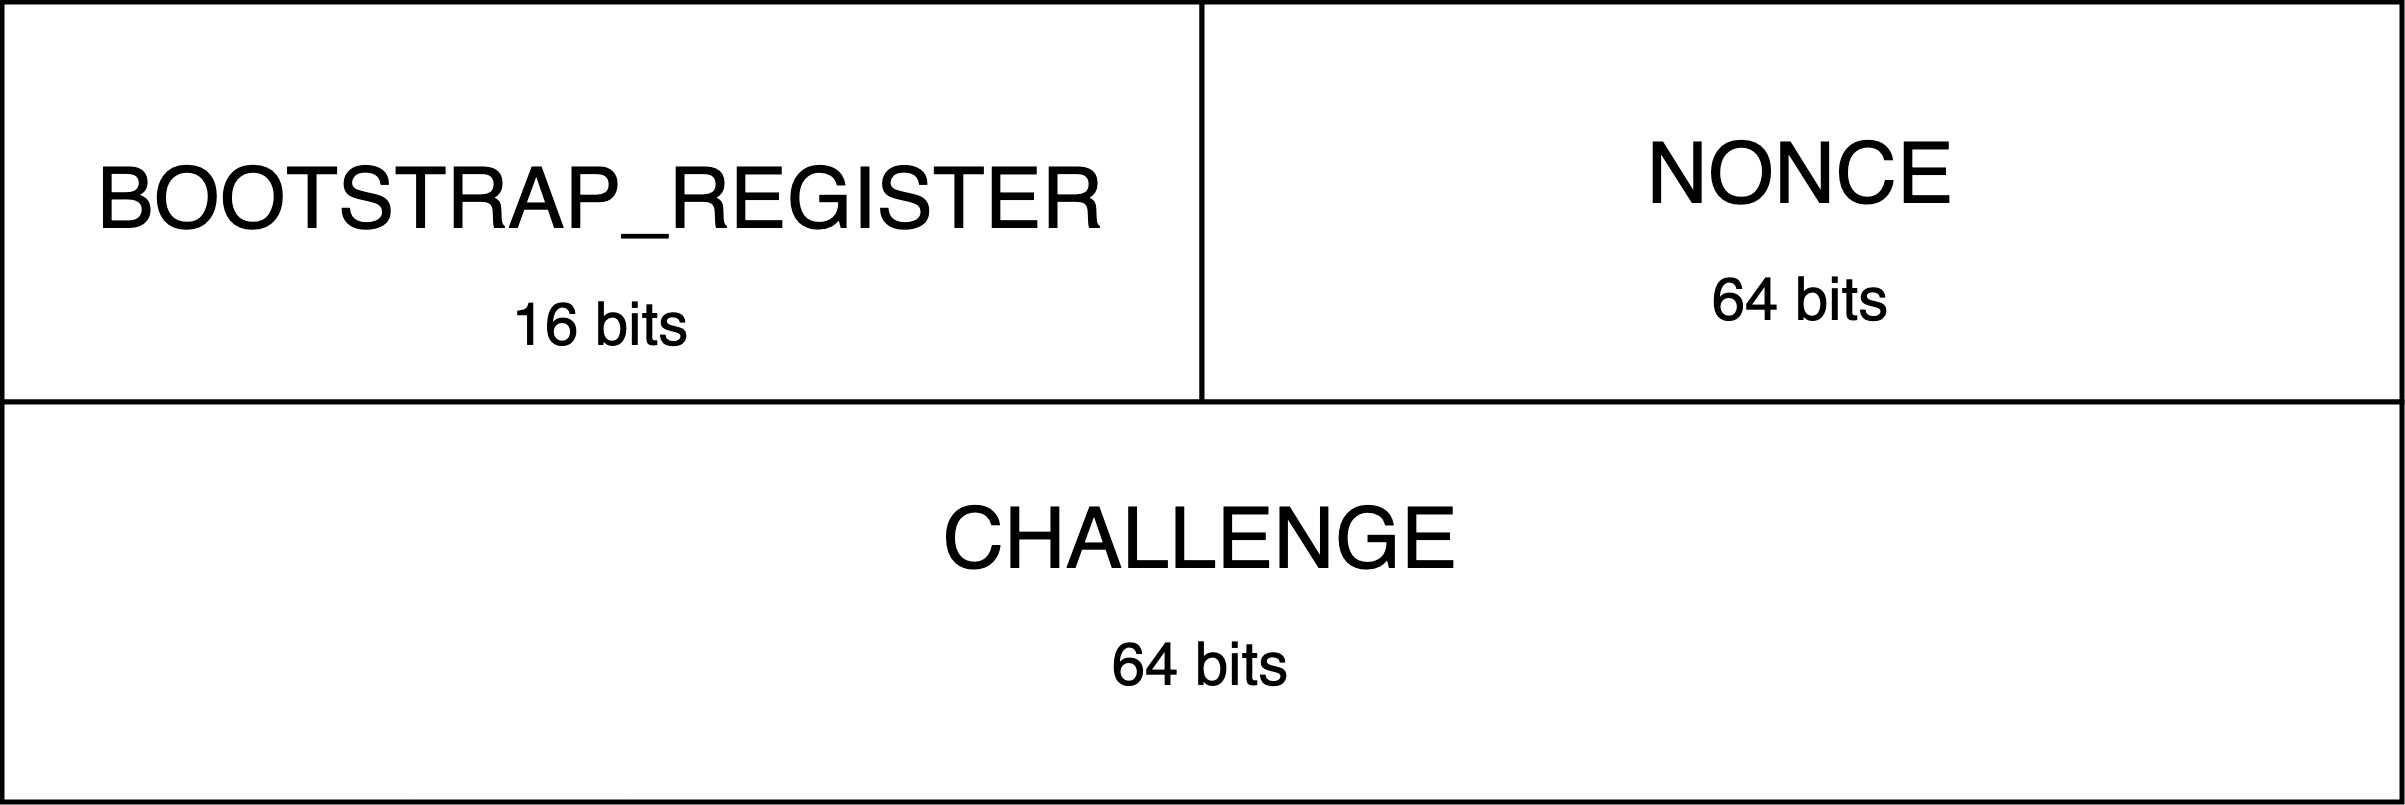
\includegraphics[width=0.45\textwidth]{pics/bootstrap.success.png}
    \caption{Bootstrap Success Message}
\end{figure}

\subsubsection{BOOTSTRAP FAILURE}
If registeration is unsuccesful, a \texttt{BOOTSTRAP\_FAILURE} message is returned to the peer with error message. 

\begin{figure}[H]
    \centering
    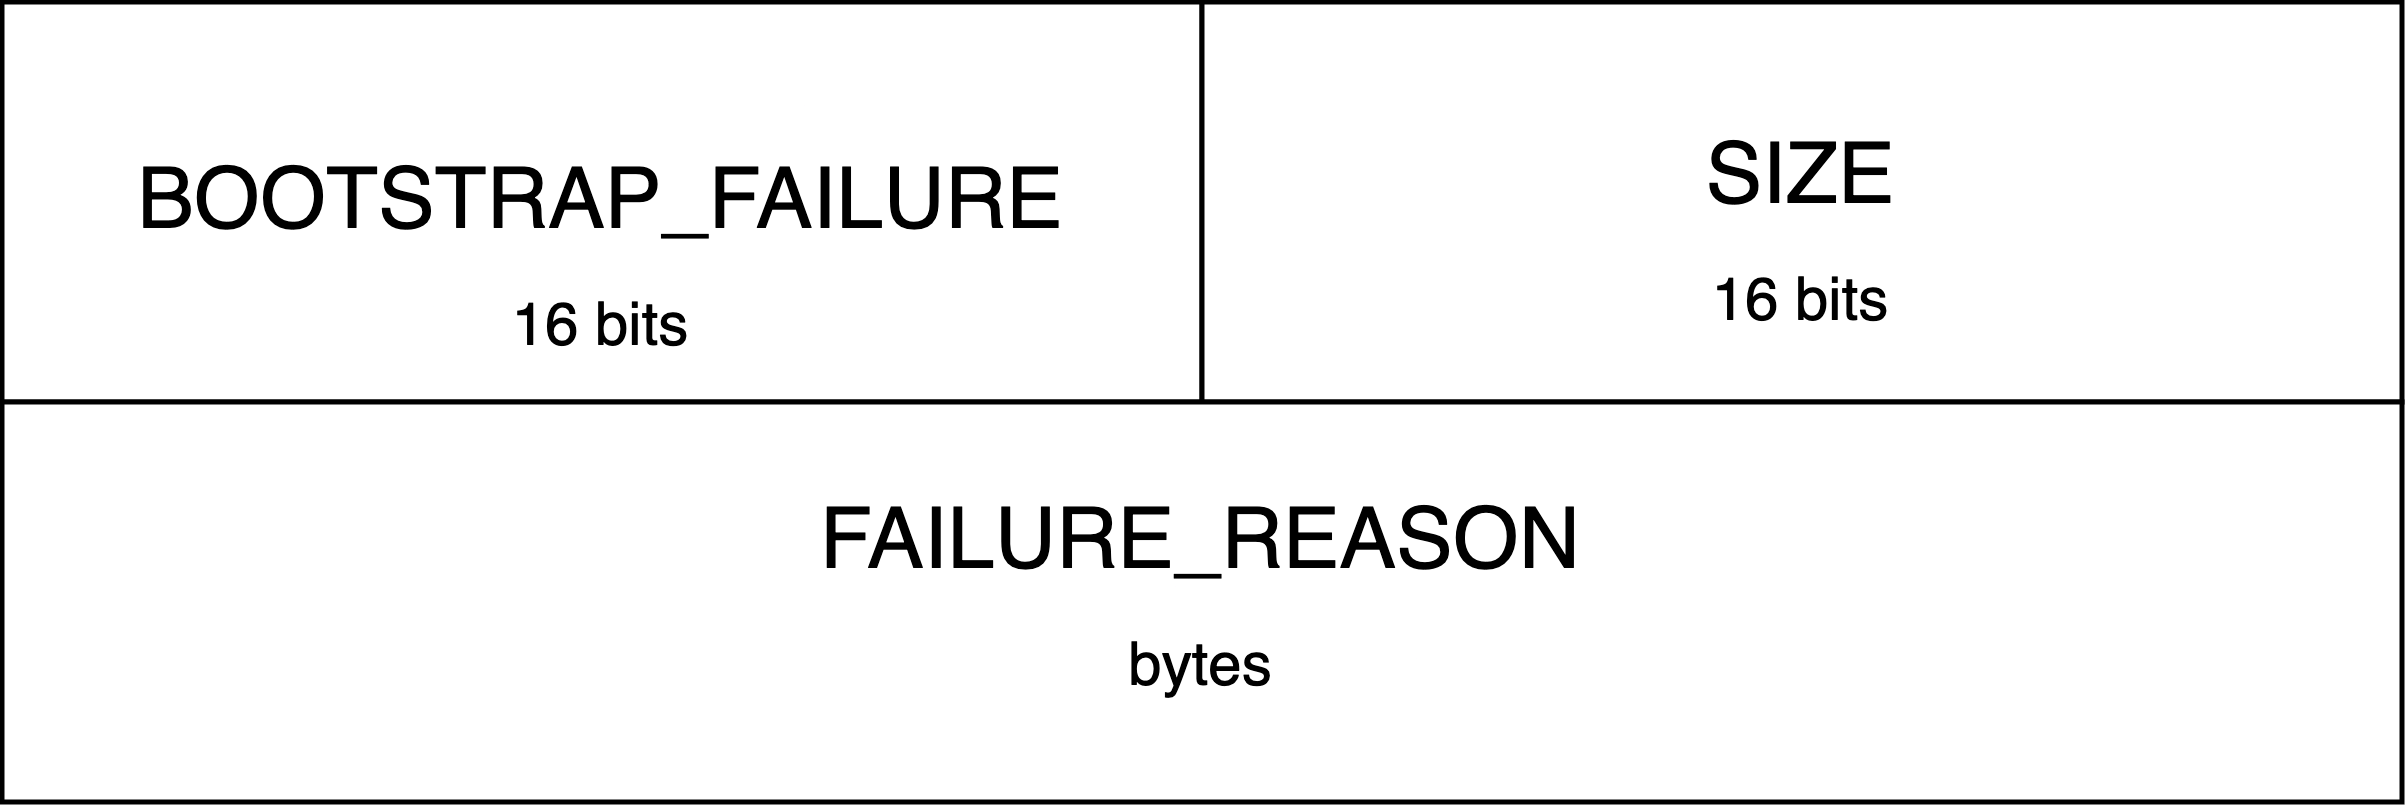
\includegraphics[width=0.45\textwidth]{pics/bootstrap.failure.png}
    \caption{Bootstrap Failure Message}
\end{figure}

\subsection{P2P}

To guarantee confidentiality, the payload data sent from peer to peer is encrypted with the public key associated with the receiving peer, which is exchanged while bootstrapping. We are currently evaluating the possibility of introducing a secure channel for the peer-to-peer connection. However, we need to assess whether we have the necessary resources and time to accomplish this.

\section{Specification of the peer-to-peer protocol that will be implemented}

\subsection{Message Types}

504: BOOTSTRAP\_INIT

505: BOOTSTRAP\_REGISTER

506: BOOTSTRAP\_SUCCESS

507: BOOTSTRAP\_FAILURE


508: PLACE\_HOLDER

509: PLACE\_HOLDER


510: DATA\_SPREAD

511: PEER\_ANNOUNCE

512: PEER\_LEAVE

513: PEER\_LIST\_REQUEST

514: PEER\_LIST\_RESPONSE


\section{Future Work}

In the upcoming weeks, there are still a few missing functionalities that need to be implemented:

\begin{itemize}
    \item \textbf{Gossip Message Handler in GossipNode}: Implement a handler that can pick up the message type from a gossip message and handle it accordingly.
    \item \textbf{Peer List Sharing Between Nodes}: Develop functionality for periodic peer list exchange to maintain up-to-date network knowledge.
    \item \textbf{Bootstrap Server to Ping Nodes}: Add a feature in the bootstrap server to ping nodes periodically to check for their vitality.
    \item \textbf{Node Join/Leave Announcements}: Ensure that nodes announce their presence when joining and notify the network when they leave.
    \item \textbf{Further Security Measures}: Implement additional security measures to enhance the robustness and security of the P2P network.
\end{itemize}

In the upcoming weeks, there are still a few missing functionalities

\section{Workload distributed}

The initial distribution works out very well as we are responsible for each part as following: Duc Trung Nguyen (design and implement P2P Protocols, including bootstrapping mechanism), Thua Duc Nguyen (implement API server, design overall architecture of the Peer, and security measurement). We will continue with that strategy.


\section{Effort spent for the project}

Throughout the project, we maintained regular communication and coordination to ensure that each team member was contributing equally. Weekly meetings were held to discuss progress, allocate tasks, and address any challenges faced. This collaborative approach allowed us to leverage each member's strengths and work effectively as a team.

The project was a result of the collective effort of all team members, with each individual contributing equally to its success.